\documentclass{article}
\usepackage{graphicx, tikz-cd, float, titlepic, booktabs} % Required for inserting images
\usepackage{pgfplots}
\usepackage{multicol}
\usepackage{makecell}
\pgfplotsset{compat=1.15}
\usepackage{mathrsfs}
\usetikzlibrary{arrows}
\usepackage{amsmath, amssymb, amsthm, amsfonts, siunitx, physics, gensymb}
\AtBeginDocument{\RenewCommandCopy\qty\SI}
\usepackage[version=4]{mhchem}
\usepackage[most,many,breakable]{tcolorbox}
\usepackage{xcolor, fancyhdr, varwidth}
\usepackage[Glenn]{fncychap}
%Options: Sonny, Lenny, Glenn, Conny, Rejne, Bjarne, Bjornstrup
\usepackage{hyperref, cleveref}
\usepackage{icomma, enumitem} %comma as decimal and continue enumerate with [resume]
\usepackage{plimsoll} %use standard state symbol with \stst
\usepackage[danish]{babel}
\renewcommand{\cellalign}{cl}
\renewcommand{\theadalign}{cl}
\renewcommand\theadfont{\bfseries}
%%%%%%%%%%%%%%%%%%%%%%%%%%%%%%
% SELF MADE COLORS
%%%%%%%%%%%%%%%%%%%%%%%%%%%%%%
\definecolor{myg}{RGB}{56, 140, 70}
\definecolor{myb}{RGB}{45, 111, 177}
\definecolor{myr}{RGB}{199, 68, 64}
\definecolor{mytheorembg}{HTML}{F2F2F9}
\definecolor{mytheoremfr}{HTML}{00007B}
\definecolor{mylenmabg}{HTML}{FFFAF8}
\definecolor{mylenmafr}{HTML}{983b0f}
\definecolor{mypropbg}{HTML}{f2fbfc}
\definecolor{mypropfr}{HTML}{191971}
\definecolor{myexamplebg}{HTML}{F2FBF8}
\definecolor{myexamplefr}{HTML}{88D6D1}
\definecolor{myexampleti}{HTML}{2A7F7F}
\definecolor{mydefinitbg}{HTML}{E5E5FF}
\definecolor{mydefinitfr}{HTML}{3F3FA3}
\definecolor{notesgreen}{RGB}{0,162,0}
\definecolor{myp}{RGB}{197, 92, 212}
\definecolor{mygr}{HTML}{2C3338}
\definecolor{myred}{RGB}{127,0,0}
\definecolor{myyellow}{RGB}{169,121,69}
\definecolor{myexercisebg}{HTML}{F2FBF8}
\definecolor{myexercisefg}{HTML}{88D6D1}
%%%%%%%%%%%%%%%%%%%%%%%%%%%%%%%%%%%%%%%%%%%%%%%%%%%%%%%%%%%%%%%%%%%%%%
% Box environments for theorems and problems
%%%%%%%%%%%%%%%%%%%%%%%%%%%%%%%%%%%%%%%%%%%%%%%%%%%%%%%%%%%%%%%%%%%%%
\setlength{\parindent}{1cm}
%================================
% Question BOX
%================================
\makeatletter
\newtcbtheorem{question}{Opgave}{enhanced,
	breakable,
	colback=white,
	colframe=myb!80!black,
	attach boxed title to top left={yshift*=-\tcboxedtitleheight},
	fonttitle=\bfseries,
	title={#2},
	boxed title size=title,
	boxed title style={%
			sharp corners,
			rounded corners=northwest,
			colback=tcbcolframe,
			boxrule=0pt,
		},
	underlay boxed title={%
			\path[fill=tcbcolframe] (title.south west)--(title.south east)
			to[out=0, in=180] ([xshift=5mm]title.east)--
			(title.center-|frame.east)
			[rounded corners=\kvtcb@arc] |-
			(frame.north) -| cycle;
		},
	#1
}{def}
\makeatother
%================================
% DEFINITION BOX
%================================

\newtcbtheorem[number within=section]{definition}{Definition}{enhanced,
	before skip=2mm,after skip=2mm, colback=red!5,colframe=red!80!black,boxrule=0.5mm,
	attach boxed title to top left={xshift=1cm,yshift*=1mm-\tcboxedtitleheight}, varwidth boxed title*=-3cm,
	boxed title style={frame code={
					\path[fill=tcbcolback]
					([yshift=-1mm,xshift=-1mm]frame.north west)
					arc[start angle=0,end angle=180,radius=1mm]
					([yshift=-1mm,xshift=1mm]frame.north east)
					arc[start angle=180,end angle=0,radius=1mm];
					\path[left color=tcbcolback!60!black,right color=tcbcolback!60!black,
						middle color=tcbcolback!80!black]
					([xshift=-2mm]frame.north west) -- ([xshift=2mm]frame.north east)
					[rounded corners=1mm]-- ([xshift=1mm,yshift=-1mm]frame.north east)
					-- (frame.south east) -- (frame.south west)
					-- ([xshift=-1mm,yshift=-1mm]frame.north west)
					[sharp corners]-- cycle;
				},interior engine=empty,
		},
	fonttitle=\bfseries,
	title={#2},#1}{def}

%================================
% NOTE BOX
%================================

\usetikzlibrary{arrows,calc,shadows.blur}
\tcbuselibrary{skins}
\newtcolorbox{note}[1][]{%
	enhanced jigsaw,
	colback=gray!20!white,%
	colframe=gray!80!black,
	size=small,
	boxrule=1pt,
	title=\textbf{Note:},
	halign title=flush center,
	coltitle=black,
	breakable,
	drop shadow=black!50!white,
	attach boxed title to top left={xshift=1cm,yshift=-\tcboxedtitleheight/2,yshifttext=-\tcboxedtitleheight/2},
	minipage boxed title=1.5cm,
	boxed title style={%
			colback=white,
			size=fbox,
			boxrule=1pt,
			boxsep=2pt,
			underlay={%
					\coordinate (dotA) at ($(interior.west) + (-0.5pt,0)$);
					\coordinate (dotB) at ($(interior.east) + (0.5pt,0)$);
					\begin{scope}
						\clip (interior.north west) rectangle ([xshift=3ex]interior.east);
						\filldraw [white, blur shadow={shadow opacity=60, shadow yshift=-.75ex}, rounded corners=2pt] (interior.north west) rectangle (interior.south east);
					\end{scope}
					\begin{scope}[gray!80!black]
						\fill (dotA) circle (2pt);
						\fill (dotB) circle (2pt);
					\end{scope}
				},
		},
	#1,
}
%================================
% EXAMPLE BOX
%================================
\newtcbtheorem[number within=section, use counter from=definition]{Example}{Example}
{%
	colback = myexamplebg
	,breakable
	,colframe = myexamplefr
	,coltitle = myexampleti
	,boxrule = 1pt
	,sharp corners
	,detach title
	,before upper=\tcbtitle\par\smallskip
	,fonttitle = \bfseries
	,description font = \mdseries
	,separator sign none
	,description delimiters parenthesis
}
{ex}
%================================
% THEOREM BOX
%================================

\tcbuselibrary{theorems,skins,hooks}
\newtcbtheorem[number within=section, use counter from=definition]{Theorem}{Theorem}
{%
	enhanced,
	breakable,
	colback = mytheorembg,
	frame hidden,
	boxrule = 0sp,
	borderline west = {2pt}{0pt}{mytheoremfr},
	sharp corners,
	detach title,
	before upper = \tcbtitle\par\smallskip,
	coltitle = mytheoremfr,
	fonttitle = \bfseries\sffamily,
	description font = \mdseries,
	separator sign none,
	segmentation style={solid, mytheoremfr},
}
{th}

%%%%%%%%%%%%%%%%%%%%%%%%%%%%%%%%%%%%%%%%%%%%%%%%%%%%%%%%%%%%%%%%%
% SELF MADE COMMANDS
%%%%%%%%%%%%%%%%%%%%%%%%%%%%%%
\newcommand{\sol}{\setlength{\parindent}{0cm}\textbf{\textit{Løsning:}}\setlength{\parindent}{1cm}}
%%%%%%%%%%%%%%%%%%%%%%%%%%%%%%%%%
\usepackage[tmargin=2cm,rmargin=1in,lmargin=1in,margin=0.85in,bmargin=2cm,footskip=.2in]{geometry}\pagestyle{fancy}
\lhead{Minrui Kevin Zhou 3.b}
\rhead{Terminsprøve}

\title{Terminsprøve\\
{\Large \textbf{Matematik A}}}
\date{\today}

\begin{document}
\maketitle
\newpage
\begin{question*}{9 - Normalfordelt fårevægt}{}
  En fåreavler har vejet sine voksne får.
  I en model kan måleresultaterne beskrives ved en stokastisk variabel $X$.
\end{question*}
\sol \\
\textbf{a.}
For at redegøre for, at $X$ tilnærmelsesvist er normalfordelt, tegner vi et fraktilplot med de givne data, hvilket ses i \cref{fig:fraktil}. 
\begin{figure}[H]
\begin{center}
  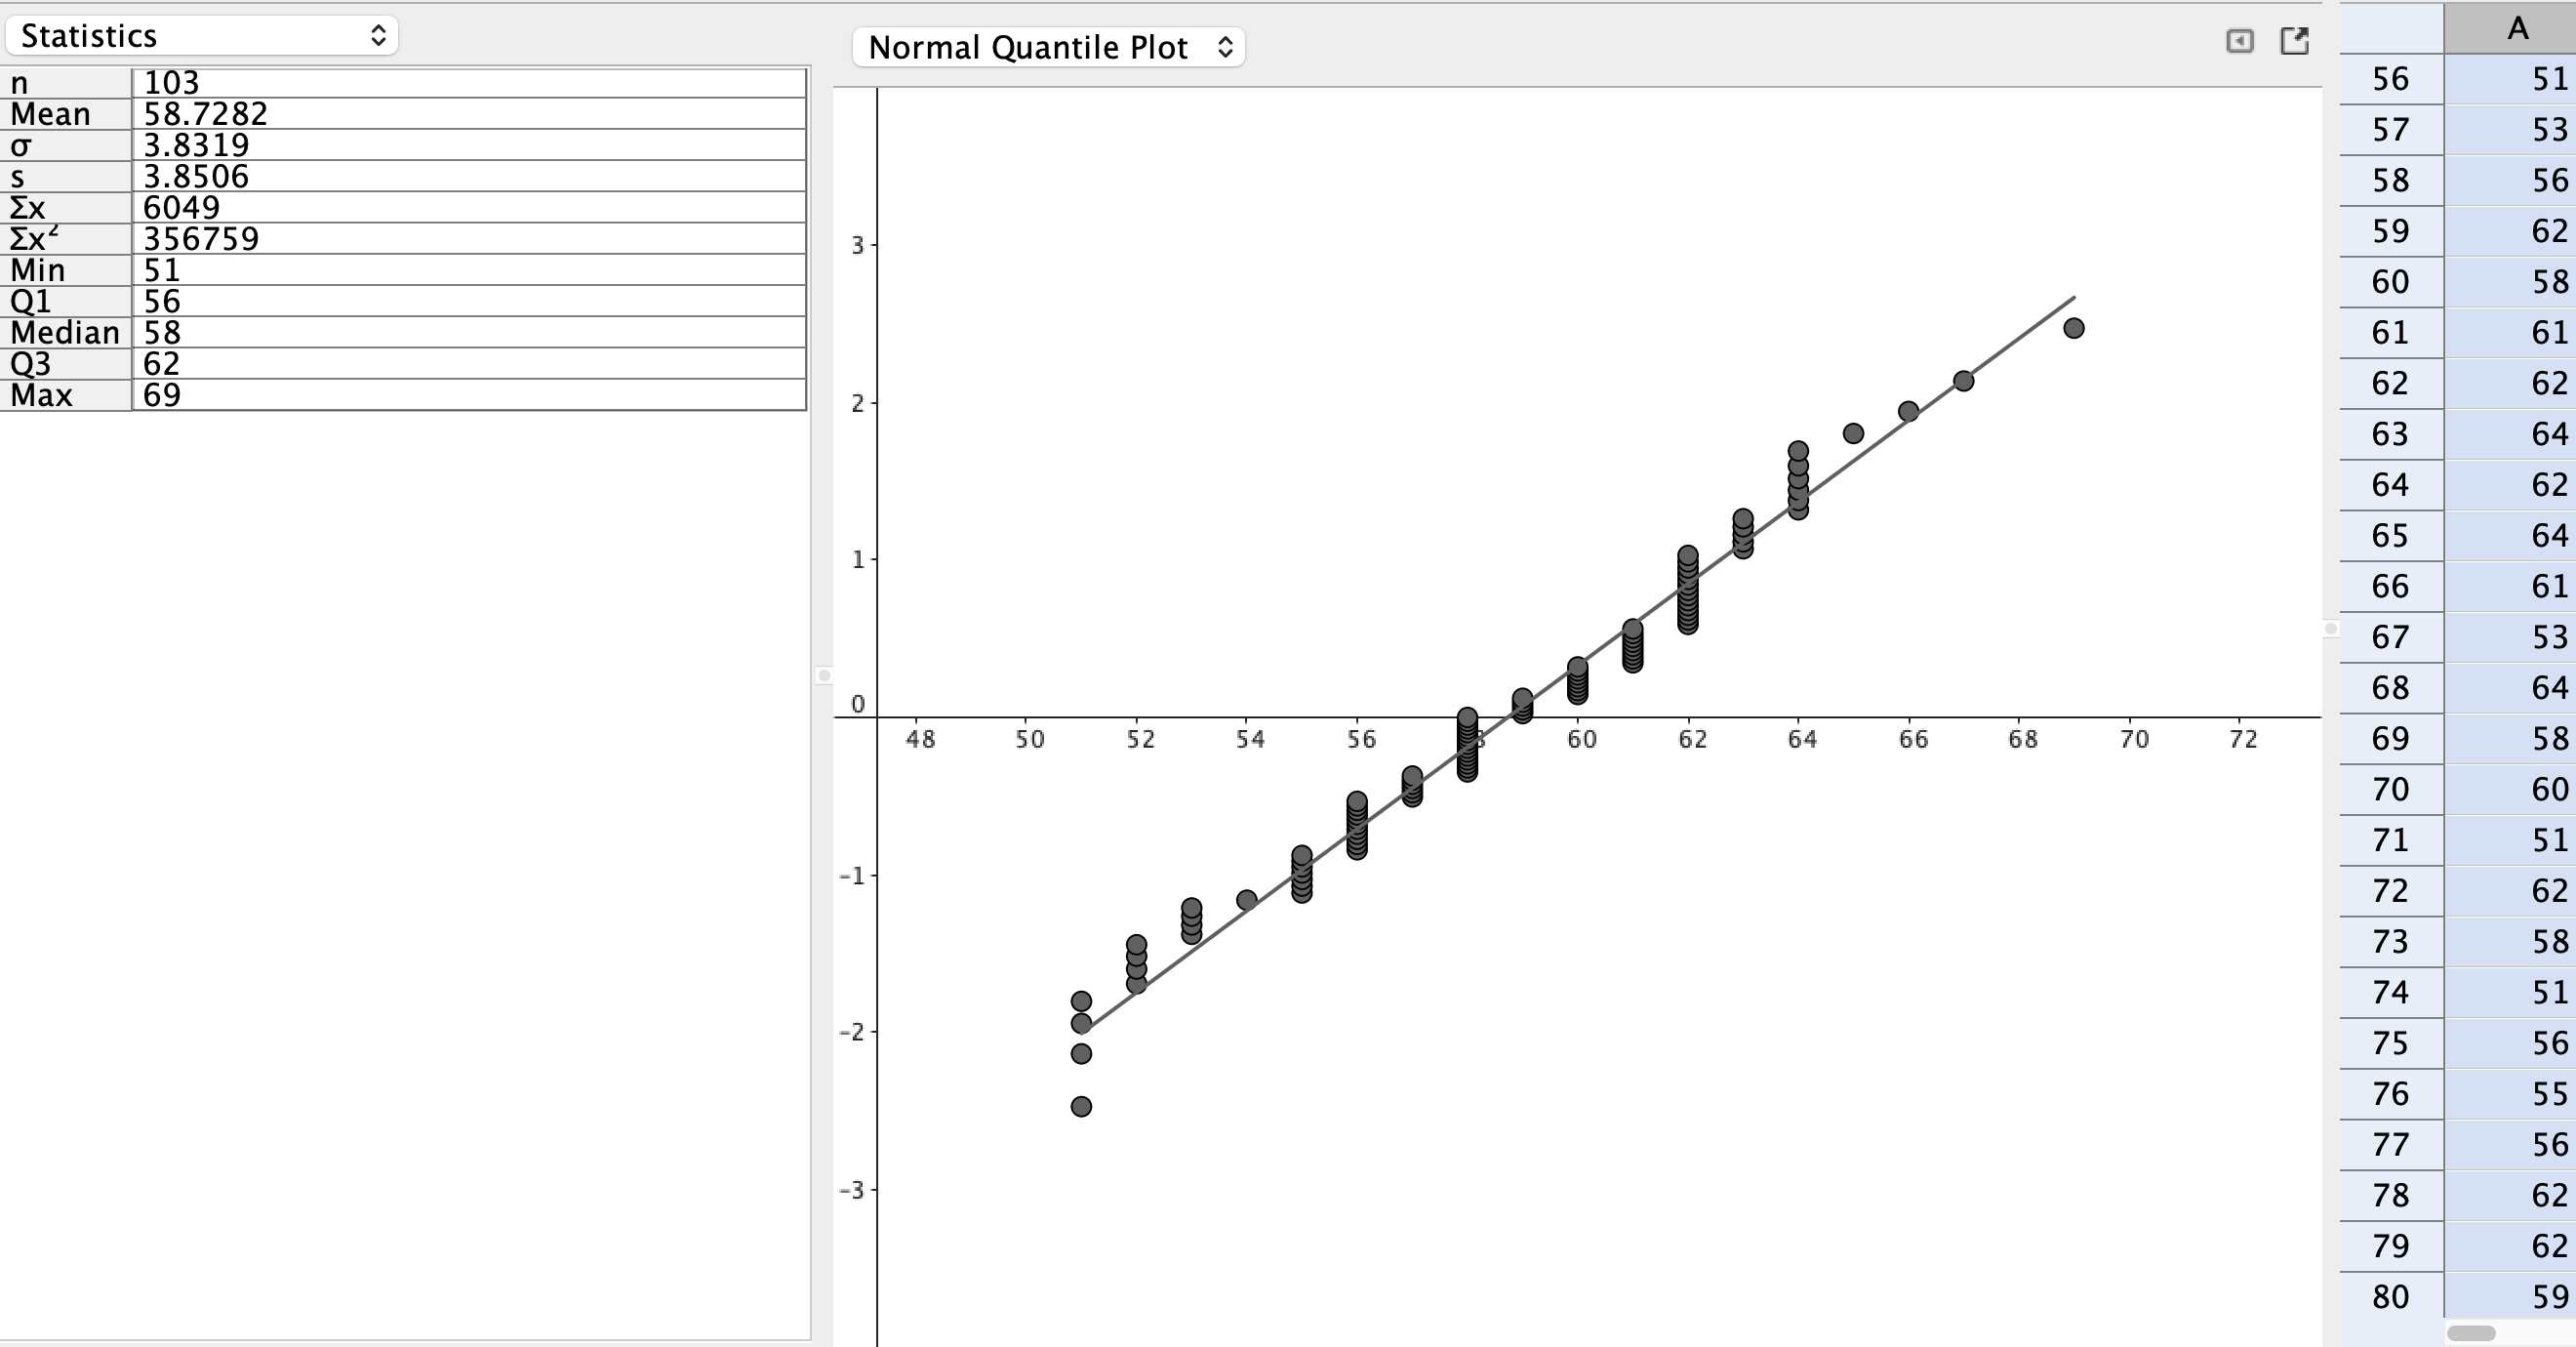
\includegraphics[width=0.7\textwidth]{fraktil.png}
\end{center}
\caption{Fraktilplot tegnet i GeoGebra}
\label{fig:fraktil}
\end{figure}
Det ses, at punkterne ligger tilnærmelsesvist på den rette linje.
Altså er $X$ tilnærmelsesvist normalfordelt med middelværdi $\mu =58,7282$ og spredning $\sigma = 3,8319$. \\[1ex]
\textbf{b.}
Vi beregner sandsynligheden med CAS, hvilket ses i \cref{fig:CASfår}.
\begin{equation*}
\begin{split}
  P(59 \leq X \leq 61) &= \Phi \left(\frac{61-58,7282}{3,8319}\right) - \Phi \left(\frac{59-58,7282}{3,8319}\right) \\
  &\approx 0,1951 \\
  &=19,51 \;\%
\end{split}
\end{equation*}
Sandsynligheden for, at et voksent får vejer mellem 59 kg og 61 kg er altså $19,51 \;\%$.
\begin{question*}{10 - Omdrejningslegeme}{}
Funktionen $f$ er givet ved
\[
f(x) = k - x^4, \quad \text{hvor } k > 0.
\] 
Grafen for $f$ afgrænser sammen med koordinatsystemets førsteakse et område $M$.
Når $M$ roteres 360° om førsteaksen dannes et omdrejningslegeme.
\end{question*}
\sol \\
\textbf{a.}
For at finde omdrejningslegemets volumen finder vi først $x$-værdierne for grafen for $f$'s skæringspunkter med førsteaksen, når $k=1$.
\begin{equation*}
\begin{split}
  f(x)= 0 &\iff 1-x^4 =0 \\
  &\iff x^4=1 \\
  &\iff x=-1 \lor x=1
\end{split}
\end{equation*}
Rumfanget af omdrejningslegemt bliver så
\begin{equation*}
\begin{split}
  V&=\pi \int_{-1}^{1} f(x)^2 \,dx \\
  &= \pi \int_{-1}^{1} \left(1-x^4\right)^2 \,dx \\
  &=\pi \int_{-1}^{1} \left(x^8+1-2x^4\right)  \,dx \\
  &= \pi \cdot \left[\frac{1}{9} \cdot x^9 + x - \frac{2}{5} x^5\right]_{-1}^{1}\\
  &=\frac{64}{45} \pi 
\end{split}
\end{equation*}
Når $k=1$ er rumfanget af omdrejningslegemet altså $\frac{64}{45} \pi $.\\[1ex]
\textbf{b.}
For at bestemme $k$, så rumfanget af omdrejningslegemet er 1000, løser vi ligningen $V=1000$ mht. $k$. 
\begin{equation*}
\begin{split}
  V=\pi \int_{-1}^{1} \left(k-x^4\right) ^2 \,dx =1000 &\iff \pi \int_{-1}^{1} \left(x^8+k^2-2x^4 \cdot k\right)  \,dx=1000\\
  &\iff \pi \cdot \left[\frac{1}{9} \cdot x^9 + k^2 \cdot x - \frac{2k}{5} x^5\right]_{-1}^{1} =1000\\
  &\implies k \approx 1,92
\end{split}
\end{equation*}
Bemærk, at vi kun den positive løsning til andengradsligningen bruges, da $k>0$.
Ligningen er løst med CAS, hvilket ses i \cref{fig:CASomdrej}.
Altså skal $k$ være $1,92$, for at rumfanget af omdrejningslegemet er 1000. 
\begin{figure}[H]
\begin{center}
  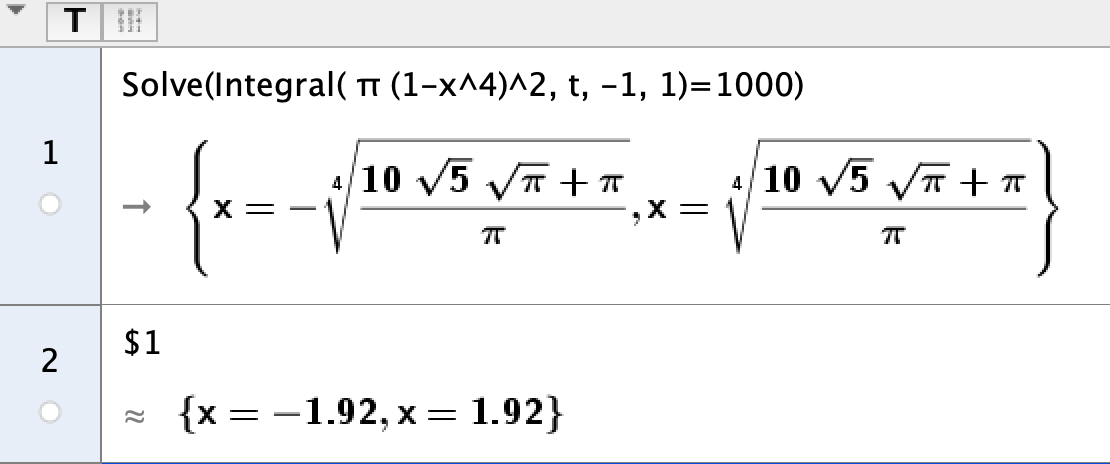
\includegraphics[width=0.7\textwidth]{CASomdrej.png}
\end{center}
\caption{Ligningen løst med CAS}
\label{fig:CASomdrej}
\end{figure}
\begin{question*}{11 - Væske i beholder}{}
I en model for tømning af væske fra en bestemt beholder kan væskehøjden beskrives ved differentialligningen
\[
  \dv{h}{t}=-16 \cdot h(t)^{-\frac{3}{2}}
\] 
hvor $h(t)$ er væskehøjden målt i cm, når der er gået t sekunder siden tømningens start.
Når tømningen startes, er væskehøjden 50 cm.
\end{question*}
\sol \\
\textbf{a.}
Siden $t=0$ ved tømningens fart, så må hastigheden, som væskehøjden falder med til start være
\begin{equation*}
\begin{split}
  h'(0)&=-16 \cdot h(0) ^{-\frac{3}{2}}\\
  &=-16 \cdot 50 ^{-\frac{3}{2}}\\
  &\approx -0,0453
\end{split}
\end{equation*}
Hastigheden, som væskehøjden falder med til start er altså $0,0453$ cm per sekund. \\[1ex]
\textbf{b.}
Vi løser differentialligningen ved seperation af variable.
\begin{equation*}
\begin{split}
  \dv{h}{t}=-16 \cdot h ^{-\frac{3}{2}} &\iff \int \frac{1}{h ^{-\frac{3}{2}}} \,dh = \int \left(-16\right)  \,dt \\
  &\iff \int h ^{\frac{3}{2}} \,dh =-16 t + c_1 \\
  &\iff \frac{2}{5} \cdot h ^{\frac{5}{2}} = -16t + c_2 \\
  &\iff h=\left(\frac{5 \cdot (-16t + c_2)}{2}\right)^{\frac{2}{5}} \\
  &\iff h=\left(-40 t + k\right) ^{\frac{2}{5}} 
\end{split}
\end{equation*}
Da vi ved, at $h(0)=5$, kan vi udregne $k$.
\begin{equation*}
\begin{split}
  h(0)=5 &\iff \left(-40 \cdot 0 + k\right) ^{\frac{2}{5}} =5 \\
  &\iff k=\pm \sqrt{5^5} \\
  &\iff k=-25 \sqrt{5}  \lor k = 25 \sqrt{5} 
\end{split}
\end{equation*}
Vi benytter den positive $k$, da væskehøjden skal falde til start.
En forskrift for $h(t)$ er altså
\[
h(t)=\left(40 \cdot t + 25 \sqrt{5} \right) ^{\frac{2}{5}}
\] 
En mulig definitionsmængde er $\mathbb{R}$.\\[1ex]
\textbf{c.}
For at finde, hvor lang tid der går, før beholderen er tom, løser vi ligningen $h(t)=0$.
\begin{equation*}
\begin{split}
  h(t)=0 &\iff (40 \cdot t + 25 \sqrt{5} ) ^{\frac{2}{5}} =0\\
  &\iff x=5 \cdot \frac{\sqrt{5} }{8} \approx 11,4
\end{split}
\end{equation*}
Ligningen er løst med CAS, hvilket ses i \cref{fig:CAStom}.
Ifølge modellen er beholderen altså tom efter 1,4 sekunder.
\begin{figure}[H]
\begin{center}
  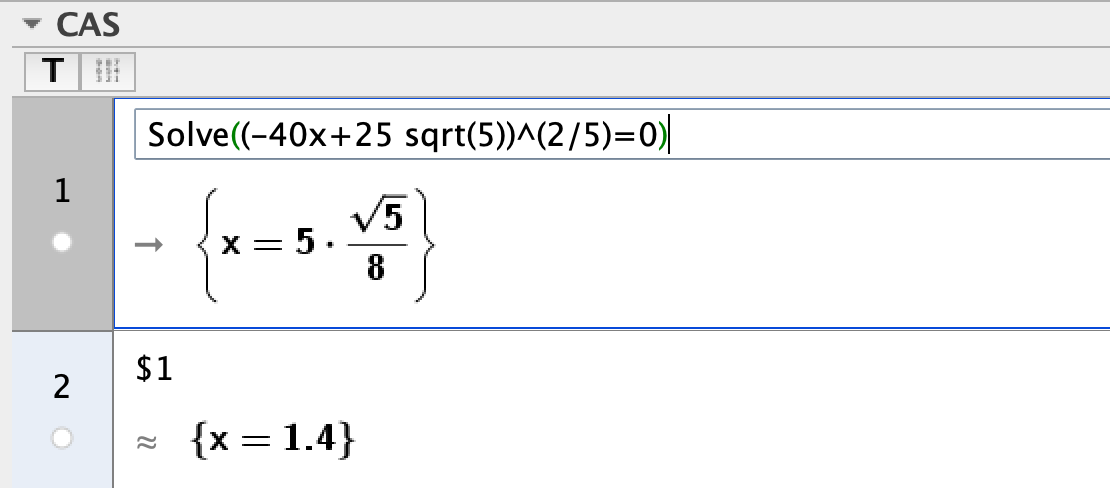
\includegraphics[width=0.7\textwidth]{CAStom.png}
\end{center}
\caption{Ligningen løst mec CAS}
\label{fig:CAStom}
\end{figure}
\begin{question*}{12 - Skøjteløber}{}
En skøjteløbers position i et koordinatsystem er givet ved vektorfunktionen
\[
  \va{s} (t)=\mqty(e^{-0,05t} \cdot \sin\left(0,5t\right) \\ e^{-0,05t} \cdot \sin\left(t\right) ), \quad t \in [0;2 \pi ]
\] 
Begge koordinatfunktioner er målt i meter, og tiden $t$ er målt i sekunder.
\end{question*}
\sol \\
\textbf{a.}
Skøjteløberens banekurve tegnet i et koordinatsystem ses i \cref{fig:skøjt}.
\begin{figure}[H]
\begin{center}
  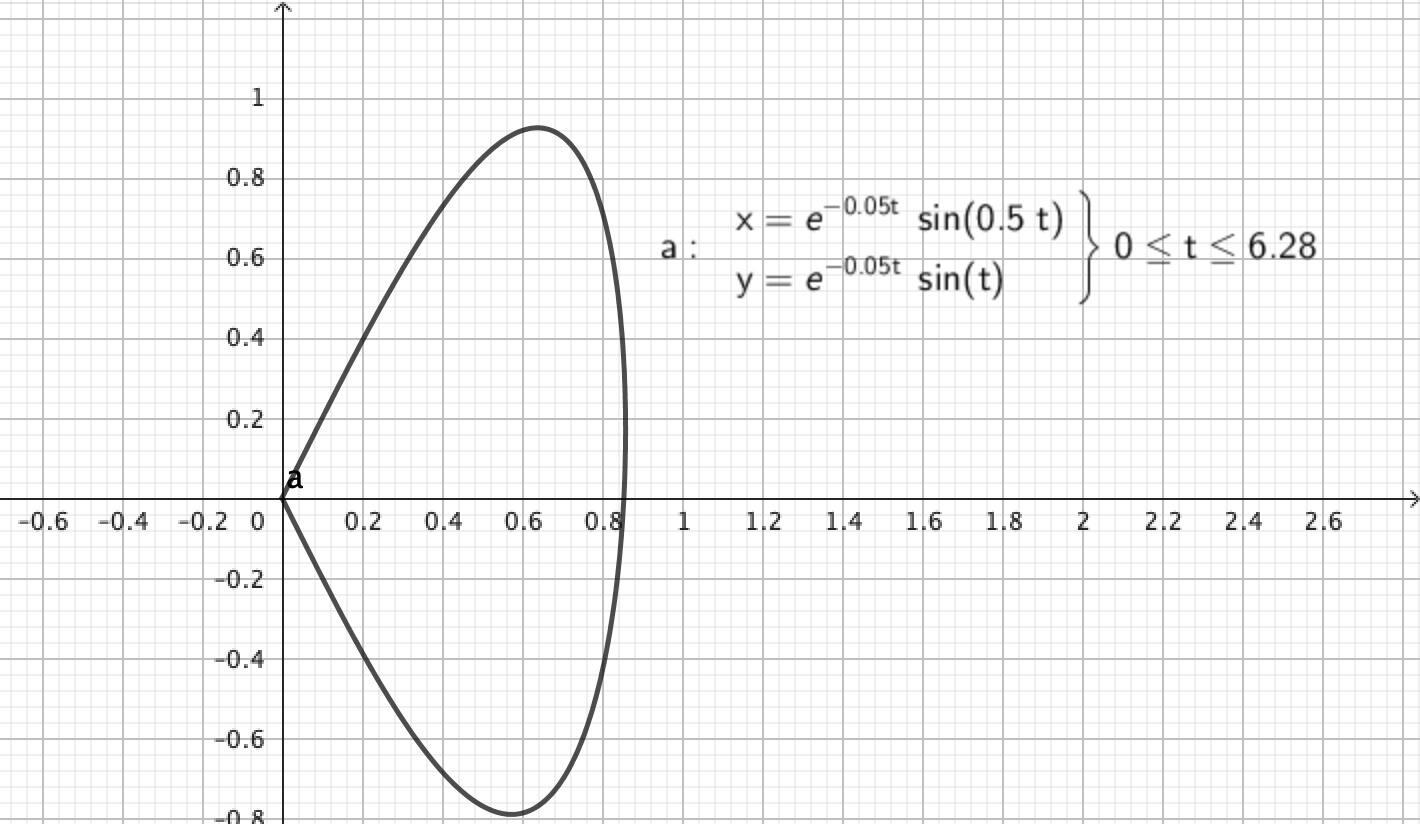
\includegraphics[width=0.7\textwidth]{skøjt.png}
\end{center}
\caption{Parameterkuven for vektorfunktionen}
\label{fig:skøjt}
\end{figure}
\noindent \textbf{b.}
For at finde $t$-værdierne, hvor løberen er på $x$-aksen løser vi ligningen $x(t)=0$.
Vi løser ligningen med CAS, hvilket ses i \cref{fig:skøjtx}.
\begin{equation*}
\begin{split}
  x(t)=0 &\iff e^{-0,05t} \cdot \sin\left(0,5t\right) =0 \land 0 \leq t \leq 2 \pi \\
  &\iff t=0 \lor t= 2 \pi 
\end{split}
\end{equation*}
Altså er skøjteløberen på førsteaksen når $t=0$ eller $t=2 \pi $. 
\begin{figure}[H]
\begin{center}
  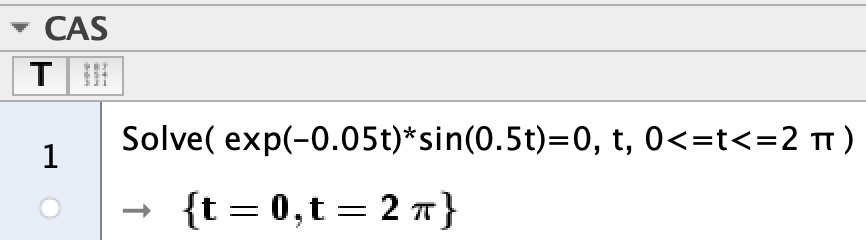
\includegraphics[width=0.7\textwidth]{skøjtx.png}
\end{center}
\caption{Ligningen løst med CAS}
\label{fig:skøjtx}
\end{figure}
\noindent \textbf{c.}
For at bestemme, hvornår størrelsen af accelerationen er maksimal, finder vi først et udtryk for skøjteløberens acceleration.
\begin{equation*}
\begin{split}
  a(t)&=\abs{\va{s}''(t)} \\
  &=\abs{\mqty(\frac{-1}{20} \; \textit{e}^{\frac{-1}{20} \; x} \; \operatorname{cos} \left( \frac{1}{2} \; x \right) - \frac{99}{400} \; \textit{e}^{\frac{-1}{20} \; x} \; \operatorname{sin} \left( \frac{1}{2} \; x \right)\\\frac{-1}{10} \; \textit{e}^{\frac{-1}{20} \; x} \; \operatorname{cos} \left( x \right) - \frac{399}{400} \; \textit{e}^{\frac{-1}{20} \; x} \; \operatorname{sin} \left( x \right)) } \\
  &=\sqrt{\left(\right)^2+\left(\right) ^2} 
\end{split}
\end{equation*}
Vi differentierer så dette udtryk og sætter lig $0$, og løser for $t$.

\begin{question*}{13 - Metalplade}{}

\end{question*}
\sol \\
\textbf{a.}
Vi bestemmer temperaturen i punktet $(-2,3)$.
\begin{equation*}
\begin{split}
  T(-2,3)&=-(-2)^2-3^2+4 \cdot \left( -2\right) -2 \cdot 3 +195 \\
  &=168
\end{split}
\end{equation*}
Temperaturen i punktet er altså $168\;\unit{\celsius} $



\end{document}
